% Mirror: https://github.com/SIGma-UIUC/presentation-format
% --------------------------------------------------------------------
% This is a simple Beamer document that uses beamerthemesigma.sty
% Reading the comments should help you create a presentation even if
% you've never used Beamer before.
% --------------------------------------------------------------------

% Set our document class to Beamer
\documentclass[handout, aspectratio=169]{beamer}
% \documentclass[aspectratio=169, handout]{beamer}
% Add handout option to ignore pauses

% From Jeff E
\usepackage{algo}
% Some more macros
\usepackage{sigmastyle}


% Set a title
\title{A Brief Introduction to Knots}

% Set a subtitle if you desire
\subtitle{}

% Whoever worked on the presentation:
\author{Jihong Cai}

% Date looks ugly, so leave blank
\date{}

% An institute name, if you're so inclined
% \institute{University of Illinois Urbana-Champaign}

% Use the SIGma theme for this Beamer presentation
\usetheme{sigma}
% --------------------------------------------------------------------

% Begin document
\begin{document}

% Beamer calls each slide a "frame", defined within the environment:
% \begin{frame}
%   <frame content here>
% \end{frame}

% This frame is just the title.
\begin{frame}
\titlepage
\end{frame}

% A frame with the table of contents.
% This frame's title is "Outline".
\begin{frame}{Outline}
  \tableofcontents
\end{frame}

\section{Basic Concepts in Topology}
\begin{frame}{What is knot? (first attempt)}
A \textbf{knot} $k:S^1\rightarrow \mathbb R^3$ is an \textbf{embedding}.

Two knots $k, l:S^1\rightarrow\mathbb R^3$ are \textbf{equivalent} if there exists an \textbf{orientation-perserving homeomorphism} between them.

A knot is called \textbf{unknot} if it is homeomorphic to $S^1$
\end{frame}

\begin{frame}{Defining Terminology}
Goal: define enough topology to understand the definitions. Here is the list:
\begin{itemize}
    \item continuous function
    \item homeomorphism
    \item embedding
    \item orientation
\end{itemize}
\end{frame}

\begin{frame}{Continuous Function}
    In topology, the only transformation we are concerned about are the continuous ones.

    In analysis, you learned that a function $f:X\rightarrow Y$ is continuous if for all $\epsilon>0$, there exists $\delta>0$ such that $|f(x)-f(y)|<\epsilon$ whenever $|x-y|<\delta$. Here $X$ and $Y$ are real lines or metric space more generally.

    Equivalently, a map $f:X\rightarrow Y$ is continuous if for any open set $U\subseteq Y$, its preimage $f^{-1}(U)$ is open in $X$.
\end{frame}
\begin{frame}{}
    \begin{center}
    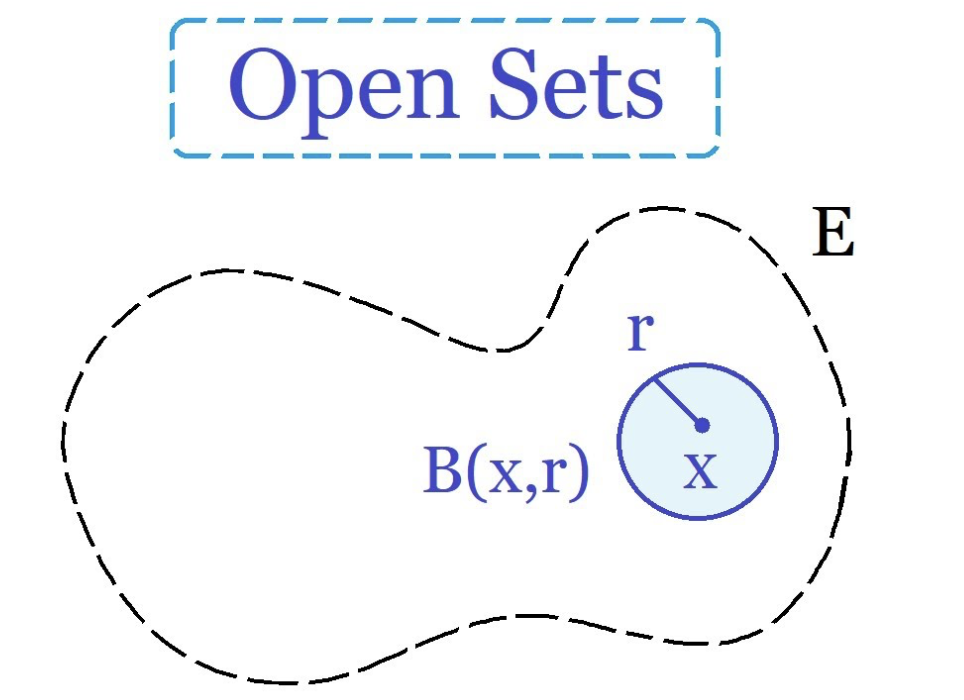
\includegraphics[scale=.5]{open set.png}
    \end{center}
\end{frame}

\begin{frame}{Homeomorphism}
    A continuous map $f: X\rightarrow Y$ is a homeomorphism if it has a continuous inverse $f^{-1}:Y\rightarrow X$.

    Equivalently, a map $f:X\rightarrow Y$ is a homeomorphism iff it is a bijective continuous open map. That means, $f$ is a bijection and
    \begin{itemize}
        \item for any open set $U\subseteq X$, $f(U)$ is open in $Y$ and 
        \item for any open set $V\subseteq Y$, $f^{-1}(U)$ is open in $X$.
    \end{itemize}
\end{frame}

\begin{frame}{Homeomorphism}
    Notice that a homeomorphism is not a continuous bijection. Here is an example:

    There is a continuous bijection $f:[0, 2\pi)\rightarrow S^1$, where
    $$S^1=\{(x,y)\in\mathbb R^2:x^2+y^2=1\}$$
    is the unit sphere.

    However, $f$ is not a homeomorphism since there is no continuous inverse. Equivalently, $f$ it is not open, since $f([0, 1))$ is not an open set in $S^1$.
\end{frame}

\begin{frame}{Embedding}
    A map $f:X\rightarrow Y$ is an embedding if $X$ and $f(X)$ are homeomorphic, i.e. there exists a homeomorphism $g:X\rightarrow f(X)$.
\end{frame}

\begin{frame}{Orientation}
I will assume the intuitive definition of orientation. A surface is orientable if ``clockwise'' or ``anti-clockwise'' direction can be defined.

For example, a Mobiüs strip is not orientable.
    
\end{frame}
\begin{frame}{Orientation}
Here is a formal definition if you wish:

Let $S$ be a surface. $S$ is orientable if its first homology group $H_1(S)$ has a trivial torsion subgroup. That means, $H_1(S)$ is a free abelian group.

$S$ is non-orientable if $H_1(S)=\mathbb Z^n+\mathbb Z/2\mathbb Z$ where $\mathbb Z^n$ is the free abelian group of rank $n$.
    
\end{frame}

\section{Knots}
\begin{frame}{What is knot? (second attempt)}
A \textbf{knot} $k:S^1\rightarrow \mathbb R^3$ is an \textbf{embedding}.

Two knots $k, l:S^1\rightarrow\mathbb R^3$ are \textbf{equivalent} if there exists an \textbf{orientation-perserving homeomorphism} between them.

A knot is called \textbf{unknot} if it is homeomorphic to $S^1$
\end{frame}

\begin{frame}{Examples of Knots}
\begin{center}
    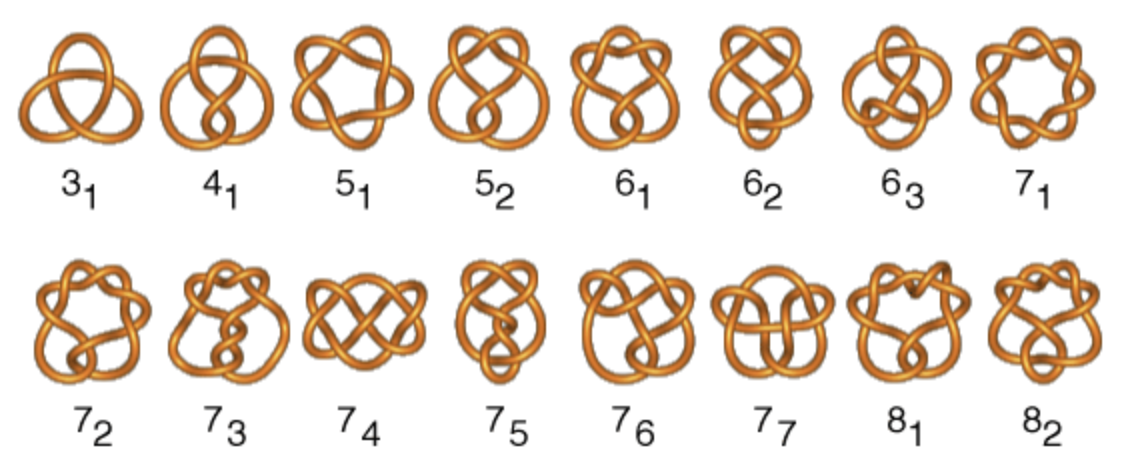
\includegraphics[scale=.5]{example.png}
\end{center}
    
\end{frame}

\begin{frame}{Why $\mathbb R^3$?}
    It is unusual for mathematician to restrict our attention to a specific space. Usually, we try to generalize things as much as possible.

    There might be two reasons behind to choice of $\mathbb R^3$:
    \begin{itemize}
        \item Embeddings in other dimensions $k:S^1\rightarrow\mathbb R^n$ ($n\neq 3$) is too hard and we cannot understand them. So we pick this special case to study first.
        \item Embeddings in other dimensions are too easy and there is not much to say about them.
    \end{itemize}
\end{frame}
\begin{frame}{Why $\mathbb R^3$?}
    \begin{theorem}
        Any embedding $f:S^1\rightarrow\mathbb R^2$ is an unknot.
    \end{theorem}
    \begin{proof}
        In $\mathbb R^2$, the knot cannot possible cross itself, so it is trivially unknotted.
    \end{proof}
\end{frame}
\begin{frame}{Why $\mathbb R^3$?}
    \begin{theorem}
        Any embedding $f:S^1\rightarrow\mathbb R^n$ for $n\geq 4$ is an unknot.
    \end{theorem}
    
\end{frame}
\begin{frame}{Higher Dimensional Knots}
    There are much to say about higher dimensional knots, but I will give a definition and a few remarks.

    A $n$-knot is an embedding $f:S^n\rightarrow\mathbb R^{n+2}$. The most common object of study is the codimension 2 knots, but I will discuss that in a bit.
\end{frame}

\begin{frame}{Higher Dimensional Knots}
    There are less tools to study knots in higher dimensions (none without introducing much more sophisticed math tools).
    
    There are two common techniques involved:
    \begin{itemize}
        \item surgery theory for geometric properties (genus) about higher dimensional knots
        \item algebraic techniques classifying knot invariants via homotopy, homology, or cohomology groups of the knot-complement (since knots themselves are always $S^n$ up to homeomorphism).
        \item differential tools in differentiable categories and PL tools in piece-wise linear categories.
        \item any combination of the above in the correct category.
    \end{itemize}
\end{frame}
\begin{frame}{Codimension Requirements for Higher Knots}
    [Zee63] and [Sta63] proved that embeddings $k: S^n \rightarrow S^m$ with codimension $m-n\geq 3$ are unknotted in the piecewise linear and topological categories.

    There is codimension $\geq 3$ knotting in the differentiable category. Differentiable embeddings $k: S^n \rightarrow S^m$ with $m - n \geq 3$ were classified by [Hae66] and [Lev65].
    
    Codimension 1 embeddings are almost as interesting as codimension 2 embeddings, although they do not have the intuitive appeal of classical knot theory. Many of the techniques used in codimension 2 make crucial use of codimension 1 embeddings, such as spanning surfaces.

\end{frame}

\section{Conclusion}
\begin{frame}{Other Interesting Structure for Knot Theorists}
\begin{itemize}
    \item Many problems about knot can be easier if we understand link. Link is an embedding $l:\coprod_{i=1}^n S^1\rightarrow \mathbb R^3$ of $n$ copies of $S^1$.
    \item Ribbon knot is also interesting, which is an immersion (self-intersection) $r:D^2\rightarrow\mathbb R^3$ with only ribbon-singularities.
\end{itemize}
\end{frame}

\begin{frame}{Connection to Other Subjects}
    \begin{itemize}
        \item knot theory as first step of proving Poincaré conjecture: property P conjecture (Dehn surgery on a knot) as a special case for the Poincaré conjecture
        \item knot theory in chemistry: study the geometric property of non-planar molecures, e.g. examining chirality via knot theory
        \item knot theory in material science: study the topological structure of materials for their physical/chemical properties, e.g. the materials and topological property of touchscreens
    \end{itemize}
\end{frame} 
\begin{frame}{Connection to Other Subjects}
    \begin{itemize}
        \item knot theory in quantum computing: redrawing quantum circuits in ZX-calculus (knot diagrams) and implement it to find better quantum algorithm.
        \item knot theory in quantum gravity: Topological Quantum Field Theory (TQFT)
        \item knot theory in particle physics: string theory
        \item complexity theory and knot theory: determining the complexity for determining if a knot is unknot
    \end{itemize}
\end{frame}
\begin{frame}[allowframebreaks]{Papers that I Mentioned}
    \tiny
    \nocite{*}
    \bibliography{refs}
    \bibliographystyle{alpha}
\end{frame}
\end{document}